\documentclass[UTF8,11pt,a4paper]{ctexart}
\usepackage[margin=2.1cm]{geometry}
\usepackage{amsmath,amssymb,booktabs,longtable,tabularx,array,multirow}
\usepackage{graphicx,float,caption,subcaption,xcolor,hyperref,enumitem}
\usepackage{siunitx}
\usepackage{fancyhdr}
\hypersetup{colorlinks=true,linkcolor=black,citecolor=black,urlcolor=blue!55!black}
\setlength{\parindent}{2em}
\setlength{\parskip}{0.16em}
\renewcommand{\arraystretch}{1.18}
\pagestyle{fancy}
\setlength{\headheight}{14pt}
\fancyhf{}
\fancyhead[C]{2018 高教社杯全国大学生数学建模竞赛 B 题：智能 RGV 的动态调度策略}
\fancyfoot[C]{\thepage}
\newcommand{\keywords}[1]{\par\noindent\textbf{关键词：}#1}
\newcommand{\argmin}{\mathop{\mathrm{arg\,min}}}
\newcommand{\E}{\mathbb E}
\newcommand{\Prob}{\mathbb P}
\title{从设备请求到可执行动作：智能 RGV 加工系统的事件驱动调度}
\author{正式竞赛长稿盲测（仅使用官方题面、附件与独立求解器）}
\date{2026 年 8 月}

\begin{document}
\maketitle

\begin{abstract}
智能加工系统中的调度并不只是在八台 CNC 中挑选一台机器。RGV 到达机器以前，CNC 可能已经完成加工；RGV 完成上下料以后，CNC 可以立即开始下一件物料，而 RGV 仍需留在原位清洗上一件成料。对于两道工序，RGV 是否携带一道工序后的半成品，又会直接改变下一时刻的候选机器集合。本文据此以事件时钟为主线，把 CNC 状态、RGV 位置、携带状态和各机器预计完成时刻放入统一状态向量，只在加工完成、故障修复或 RGV 完成一项动作时推进决策。

对一道工序情形，八台 CNC 的刀具相同，候选集合由空闲机和已完成机组成。本文比较就近优先、预计服务完成优先和带完成品偏好的平衡规则。三组参数下，三种规则在确定性情形均得到相同班产量，分别为 356、336 和 366 件；因此一道工序采用更容易复核的就近优先规则，而不把三种规则的同值误写成一般等价。对应 RGV 忙碌占比分别为 84.93\%、93.05\% 和 86.21\%，其余时间为等待 CNC 完成。

对两道工序情形，先枚举第一工序 CNC 数为 2--6 的 238 种刀具分配，再对每种分配运行三种动态规则。第 1、2 组数据均由就近优先取得较高班产量，最优分配分别为 $12121212$ 和 $21211212$，完成 235 和 202 件；第 3 组第二工序只需 182 s，固定的就近规则容易使第二工序机空等，预计服务完成优先选择 $21112121$，完成 239 件。该搜索对给定的刀具分配集合是穷举，对所有可能的动态策略并非全局最优证明。

故障情形在每次 CNC 开始加工时以 1\% 概率触发，故障发生时刻在本次加工区间内均匀抽取，修复时间在 600--1200 s 内均匀抽取。固定随机种子下，每组参数、每种工序情形独立仿真 200 次。一道工序平均班产量为 350.595、330.385 和 359.850 件；两道工序平均班产量为 228.390、189.765 和 220.990 件。第 3 组两道工序的平均损失达到 18.01 件，说明较短的第二工序并未消除故障传播：一道工序的中断会使半成品供应和 RGV 后续访问同时改变。全文保留具体调度表、候选统计、资源占比和故障损失接口，结果只对应题面参数、所列规则和 8 h 班次。

\keywords{RGV；动态调度；离散事件仿真；两阶段加工；设备故障；枚举优化}
\end{abstract}

\phantomsection\label{mcm-body-start}
\section{问题重述}

题目给出的加工系统由 8 台 CNC、1 辆带双手爪和清洗槽的 RGV、1 条直线轨道以及上下料传送带构成。CNC1/2、3/4、5/6、7/8 分别位于轨道的四个工位，RGV 初始停在 CNC1 与 CNC2 之间。每台 CNC 加工完成后发出请求；若 RGV 尚未到达，该 CNC 保持等待。RGV 同一时刻只能移动、等待、上下料或清洗，不能把这些动作同时分给两个请求。

一道工序时，八台 CNC 安装相同刀具，生料在任一 CNC 上加工后即可成为熟料。RGV 到达已完成 CNC 时，双手爪允许一次完成“卸下熟料、装入生料”；随后 CNC 可开始加工新料，RGV 则在原位完成熟料清洗并送入下料传送带。题目要求给出一般动态调度模型，并用三组移动、加工、上下料和清洗时间计算 8 h 班次内的调度与作业效率。

两道工序时，每件物料必须先后在两台不同 CNC 上加工。CNC 的刀具在班次内不更换，因而调度开始前还需确定哪些机器承担第一工序、哪些机器承担第二工序。RGV 从第一工序机卸下半成品后，在送入第二工序以前一直占用一只手爪；此时它不能再去另一台第一工序机卸出新的半成品。这个携带约束把刀具分配和访问顺序连在了一起。

故障情形中，CNC 每次加工可能以约 1\% 的概率发生故障，未完成物料报废，修复需 10--20 min，修复后机器重新加入作业序列。需要分别给出一道、两道工序下的调度结果。题面没有给出故障发生时刻的经验分布和多台机器之间的相关性，因此随机机制必须单独列为情景假设，不能与确定性结果混成一个班产量。

\section{问题分析：先分清谁在等待谁}

这道题最容易出现的偏差，不是某个启发式公式少了一项，而是把动作的并发关系写错。RGV 为已完成 CNC 上下料后，CNC 已经具备下一次加工条件；清洗发生在 RGV 上，故 CNC 加工可以与 RGV 清洗重叠。另一方面，附件明确指出清洗过程中 RGV 不能移动，所以清洗时间仍要进入 RGV 的下一次可用时刻。若把清洗加进 CNC 加工时间，机器会被无故延迟；若让 RGV 边清洗边移动，班产量又会被高估。

静态循环也不足以描述实际请求。班次开始时八台 CNC 都为空，RGV 会连续完成首轮上料；进入稳定阶段后，各 CNC 的完成时刻已经因奇偶上下料时间、移动距离和前次等待而错开。此后即使 RGV 每次采用相同的规则，访问序列也不再是固定的 $1,2,\ldots,8$。因此本文不预先生成整班路线，而是在每个决策时刻读取当前状态，再选择下一项可执行动作。

一道工序的候选关系相对简单：只要 CNC 为空或已完成，它就可以接受 RGV 服务。三个规则在对称工位和长加工时间下可能给出相同产量，但访问细节仍可不同。规则的取舍应先看班产量，再看 RGV 等待、移动和结果是否容易复算，而不能仅凭“智能”或“全局”这样的名称判断。

两道工序多了一层物料流。第一工序机器过多，第二工序会成为瓶颈；第二工序机器过多，半成品供应不足。只按加工时间比计算机器数可以给出量级，却没有计入 RGV 的移动和上下料。由于机器只有 8 台，本文直接枚举合理刀具分配，并在每个分配上运行相同的事件调度，以免先用连续比例取整后漏掉工位位置带来的差别。

故障不只是从确定性产量中减去“故障次数乘平均修复时间”。一台第一工序 CNC 停机会使半成品到达节奏改变，RGV 随后的候选集合也随之改变；两道工序中的损失不能由一道工序的比例直接平移。本文保留逐次故障仿真，报告均值、标准差和分位数，同时把无故障结果作为同策略基线。

\begin{table}[H]
\centering
\caption{三组系统参数及其在模型中的位置}
\label{tab:parameters-b}
\small
\begin{tabularx}{\textwidth}{p{4.7cm}rrrX}
\toprule
参数/s & 第1组 & 第2组 & 第3组 & 进入的模型环节\\
\midrule
移动 1/2/3 个工位 & 20/33/46 & 23/41/59 & 18/32/46 & 候选到达时刻和 RGV 忙碌时间\\
一道工序加工 & 560 & 580 & 545 & CNC 完成事件\\
第一工序加工 & 400 & 280 & 455 & 半成品产生时刻\\
第二工序加工 & 378 & 500 & 182 & 成品产生时刻\\
奇数 CNC 上下料 & 28 & 30 & 27 & 服务动作持续时间\\
偶数 CNC 上下料 & 31 & 35 & 32 & 服务动作持续时间\\
成料清洗 & 25 & 30 & 25 & 阻塞 RGV，但不阻塞已重新开工的 CNC\\
\bottomrule
\end{tabularx}
\end{table}

\section{模型假设}
\begin{enumerate}[label=\arabic*)]
\item RGV 和 CNC 在题面给出的动作时间内完成对应动作，移动和上下料之间不另加未给出的启停时间。
\item 同一工位的两台 CNC 到 RGV 轨道位置相同，四个工位依次记为 0、1、2、3；RGV 初始位置为 0。
\item 原料供应充足，下料传送带不会堵塞；一道工序后的半成品由 RGV 直接携带到第二工序机，不设额外缓存。
\item CNC 在一次上下料结束后立即开始新一轮加工。若本次卸出最终成品，RGV 随后的清洗与该 CNC 的加工并行，但 RGV 在清洗结束前不能移动。
\item 确定性情形不发生故障。故障情形下，每次开始加工独立以 0.01 概率发生故障，故障点在加工区间内均匀分布，修复时间在 600--1200 s 内均匀分布。
\item 班次在 $H=28800$ s 截止；只有清洗完成且时间不超过 $H$ 的成品计入班产量。跨越班次边界的移动、等待和清洗只计入边界以内的资源时间。
\item 本文比较的三种规则构成有限候选集。刀具分配的枚举是完整的，动态规则空间并未穷尽，故输出称为候选策略下的可行调度。
\end{enumerate}

\section{符号说明}
\begin{table}[H]
\centering
\caption{主要符号及状态量}
\label{tab:symbols-b}
\small
\begin{tabularx}{\textwidth}{p{2.4cm}p{7.2cm}p{2.1cm}X}
\toprule
符号 & 含义 & 单位 & 备注\\
\midrule
$H$ & 一个班次的截止时刻 & s & $28800$\\
$x_i$ & CNC $i$ 所在工位 & -- & $x_i=\lfloor(i-1)/2\rfloor$\\
$s_i(t)$ & CNC 状态 & -- & 空闲、加工、完成或维修\\
$r_i$ & CNC 下一次完成加工或修复的时刻 & s & 事件时钟\\
$p(t)$ & RGV 当前工位 & -- & 0--3\\
$b(t)$ & RGV 是否携带半成品 & -- & 两道工序使用\\
$z_i$ & CNC $i$ 的刀具类别 & -- & 1 为第一工序，2 为第二工序\\
$d(a,b)$ & 工位 $a$ 到 $b$ 的移动时间 & s & 由表\ref{tab:parameters-b}查得\\
$u_i$ & CNC $i$ 的一次上下料时间 & s & 奇偶编号不同\\
$c$ & 最终成品清洗时间 & s & 只清洗熟料\\
$N(H)$ & 班次内完成并清洗的成品数 & 件 & 主目标\\
$\mathcal E(t)$ & 时刻 $t$ 的可服务 CNC 集合 & -- & 随状态和携带量变化\\
\bottomrule
\end{tabularx}
\end{table}

\section{任务一模型的建立与求解：一般事件调度框架}
\label{mcm-q1-start}

\subsection{状态只在事件处更新}

把 CNC $i$ 的状态写成
\begin{equation}
s_i(t)\in\{\mathrm{empty},\mathrm{processing},\mathrm{done},\mathrm{repair}\}.
\label{eq:cnc-state-b}
\end{equation}
空闲机可以装入原料或半成品；加工机在 $r_i$ 到达以前不能服务；完成机已经发出需求；维修机要等修复时刻以后才重新变为空闲。完整系统状态记为
\begin{equation}
X(t)=\bigl(t,p(t),b(t),\{s_i(t),r_i,z_i\}_{i=1}^{8},N(t)\bigr).
\label{eq:system-state-b}
\end{equation}
其中 $b(t)$ 在一道工序时恒为 0，在两道工序时表示 RGV 手爪中是否有等待转运的半成品。

程序不按 1 s 网格逐秒扫描，而是在当前没有可执行请求时直接跳到最近的 CNC 完成或维修结束时刻：
\begin{equation}
t\leftarrow \min_{i:s_i=\mathrm{processing}} r_i.
\label{eq:event-jump-b}
\end{equation}
这样既保留了等待时间，也不会在 8 h 班次内生成大量无动作记录。若多个 CNC 同时完成，候选评分中的编号只承担最终平局规则，不改变已完成状态。

\begin{table}[H]
\centering
\caption{CNC 状态转换和触发事件}
\label{tab:state-transition-b}
\small
\begin{tabularx}{\textwidth}{p{2.2cm}p{3.4cm}p{4.3cm}X}
\toprule
原状态 & 触发条件 & 新状态与时刻 & 对候选集合的影响\\
\midrule
empty & RGV 完成上料 & processing，$r_i=t+T_i$ & 暂时移出候选集\\
processing & $t=r_i$ 且正常完成 & done & 发出上下料请求\\
processing & 故障并完成修复 & empty & 报废在制品，重新请求原料\\
done & RGV 完成上下料 & processing 或 empty & 取决于是否同时装入下一件\\
repair & 修复截止时刻到达 & empty & 重新进入候选集\\
\bottomrule
\end{tabularx}
\end{table}

\subsection{到达、等待与服务必须分开记账}

若当前 RGV 位于 $p$，候选 CNC $i$ 位于 $x_i$，移动后到达时刻为
\begin{equation}
a_i=t+d(p,x_i).
\label{eq:arrival-b}
\end{equation}
对于尚在加工但会在 RGV 到达前完成的机器，实际服务开始时刻是 $\max(a_i,r_i)$；当前实现只把已发出请求的机器放进候选集，因而加工机通常在事件跳转后才进入集合。保留 $r_i$ 项的目的，是使预计完成优先规则可以直接扩展到“提前派车”等变体，而不改状态接口。

RGV 的一次访问由移动、可能的等待、上下料和可选清洗组成。CNC 新一轮加工从上下料结束时刻开始，若卸出最终成品，RGV 再执行清洗。两个时钟因此分开更新：
\begin{align}
r_i&=t_{\mathrm{service\ end}}+T_i,\label{eq:cnc-restart-b}\\
t_{\mathrm{RGV\ next}}&=t_{\mathrm{service\ end}}+mathbf 1_{\{\mathrm{final}\}}c.
\label{eq:rgv-next-b}
\end{align}
式\eqref{eq:cnc-restart-b}和式\eqref{eq:rgv-next-b}相差一个清洗时间。这一差别虽只有 25--30 s，却会在数百次访问后累积成明显产量差。

\begin{table}[H]
\centering
\caption{RGV 动作与设备并发关系}
\label{tab:concurrency-b}
\small
\begin{tabularx}{\textwidth}{p{3.5cm}p{3.5cm}p{3.8cm}X}
\toprule
RGV 动作 & RGV 能否同时移动 & 被服务 CNC 的状态 & 其他 CNC 的状态\\
\midrule
移动到目标 CNC & 否 & 可继续加工或等待 & 各自继续加工\\
等待目标完成 & 否 & 加工至 $r_i$ & 各自继续加工\\
上下料 & 否 & 暂停，结束后可开工 & 各自继续加工\\
清洗最终成品 & 否 & 已装入新料并加工 & 各自继续加工\\
原地无请求等待 & 否 & 按各自时钟推进 & 按各自时钟推进\\
\bottomrule
\end{tabularx}
\end{table}

\subsection{三个候选评分不是三个黑箱算法}

对候选 CNC $i$，记移动时间为 $m_i=d(p,x_i)$，到达后的等待为 $w_i=\max(0,r_i-t-m_i)$。本文使用三种可以逐步复算的评分：
\begin{align}
J_i^{(N)}&=m_i+w_i,\label{eq:nearest-score-b}\\
J_i^{(E)}&=\max(t+m_i,r_i)+u_i,\label{eq:earliest-score-b}\\
J_i^{(B)}&=m_i+0.8w_i-0.35c\,\mathbf 1_{\{s_i=\mathrm{done}\}}.
\label{eq:balanced-score-b}
\end{align}
三式分别对应就近可服务、预计本次服务较早结束、以及在移动和等待接近时优先处理已完成机器。每个决策时刻取
\begin{equation}
i^*=\argmin_{i\in\mathcal E(t)}J_i,
\label{eq:dispatch-choice-b}
\end{equation}
若评分相同，再按预计完成时刻和 CNC 编号排序。系数 0.8 和 0.35 只用于构造第三个对照规则，不据此宣称已经标定出最优权重。

\begin{table}[H]
\centering
\caption{三种规则实际比较的对象}
\label{tab:policy-meaning-b}
\small
\begin{tabularx}{\textwidth}{p{3.0cm}p{4.1cm}p{4.1cm}X}
\toprule
规则 & 优先避免的损失 & 可能忽略的对象 & 本文中的用途\\
\midrule
就近优先 & 空驶和远距离往返 & 远端已完成 CNC 的等待 & 一道工序基准；第1、2组两工序候选\\
预计服务完成优先 & 当前动作结束过晚 & 频繁跨工位的后续代价 & 第3组两工序候选\\
平衡规则 & 已完成机器长期滞留 & 权重没有外部标定 & 检查简单规则是否明显漏解\\
\bottomrule
\end{tabularx}
\end{table}

\subsection{目标函数和输出边界}

主目标是在班次内最大化已完成第二工序并清洗的成品数：
\begin{equation}
\max N(H).
\label{eq:objective-b}
\end{equation}
当多个候选得到相同 $N(H)$ 时，本文不再用任意加权总分强行排出唯一名次，而是同时查看 RGV 忙碌占比、等待占比和平均 CNC 利用率。班次末仍在加工或尚未完成清洗的物料不计产量；这条边界也解释了为什么动作日志中的最后一次卸料动作可能多于计入的成品数。

算法对每个候选都保存访问起止时刻、CNC 编号、动作类型和累计成品数。正文的班产量来自日志累计值，资源占比来自截断到 $H$ 的移动、等待、上下料和清洗时长。若二者由两套循环分别生成，班次边界很容易出现一个计数包含最后一件、另一个计数排除最后一件的问题。

\label{mcm-q1-end}

\section{任务二（一）模型的建立与求解：一道工序调度}
\label{mcm-q2-start}

\subsection{从首轮上料到稳定访问}

班次开始时八台 CNC 均为空闲。RGV 的第一轮动作只包含装入生料，没有可卸下的成品，也不执行清洗。首批机器开始加工以后，后续请求由各自的完成时刻触发。候选集合写成
\begin{equation}
\mathcal E_1(t)=\{i:s_i(t)\in\{\mathrm{empty},\mathrm{done}\}\}.
\label{eq:eligible-one-b}
\end{equation}
若目标 CNC 已完成，RGV 一次上下料同时卸出成品并装入生料；CNC 随即开工，RGV 再用 $c$ 秒清洗。若目标 CNC 为空，只装入生料，不产生清洗动作。

初始阶段不能直接用于估计稳态成品间隔。第1组第一件成品在 687 s 完成，随后相邻成品间隔均值为 79.10 s；若把 687 s 的启动时间也放进间隔样本，方差会被人为放大。本文分别记录第一件、最后一件和启动后的相邻间隔，班产量仍按完整 8 h 计算。

\subsection{三种规则先全部运行，再决定保留哪一个}

一道工序中三组参数的三种规则均得到相同班产量。这个现象来自加工时间远长于单次移动和上下料，且八台 CNC 同质；它只说明在当前三个参数组与本次平局规则下，三种局部评分没有改变最终完成数。访问路径、等待位置和对其他参数的响应仍可能不同。

既然产量相同，正式方案保留就近优先。它的每一步只需比较移动和当前等待，现场实现不需要预测多步后的完成序列。若以后增加缓存上限、交货优先级或不同 CNC 加工时间，预计完成优先可能重新占优，不能把本次选择写成一道工序的一般定理。

\begin{table}[H]
\centering
\caption{一道工序确定性调度结果}
\label{tab:one-stage-results-b}
\small
\begin{tabular}{crrrr}
\toprule
参数组 & 班产量/件 & RGV忙碌占比 & RGV等待占比 & 平均CNC利用率\\
\midrule
第1组 & 356 & 0.8493 & 0.1507 & 0.8872\\
第2组 & 336 & 0.9305 & 0.0695 & 0.8685\\
第3组 & 366 & 0.8621 & 0.1379 & 0.8847\\
\bottomrule
\end{tabular}
\end{table}

第2组加工时间最长、移动和上下料也最慢，班产量降至 336 件；与此同时 RGV 忙碌占比达到 93.05\%。这并不与“加工时间长”矛盾：移动和服务时间同步增加，使 RGV 可等待的空档缩短。第3组加工时间最短且移动较快，班产量最高；RGV 仍有 13.79\% 时间在等待，说明此时不能仅通过缩短路线把产量推到加工时间给出的松弛上界。

\begin{figure}[H]
\centering
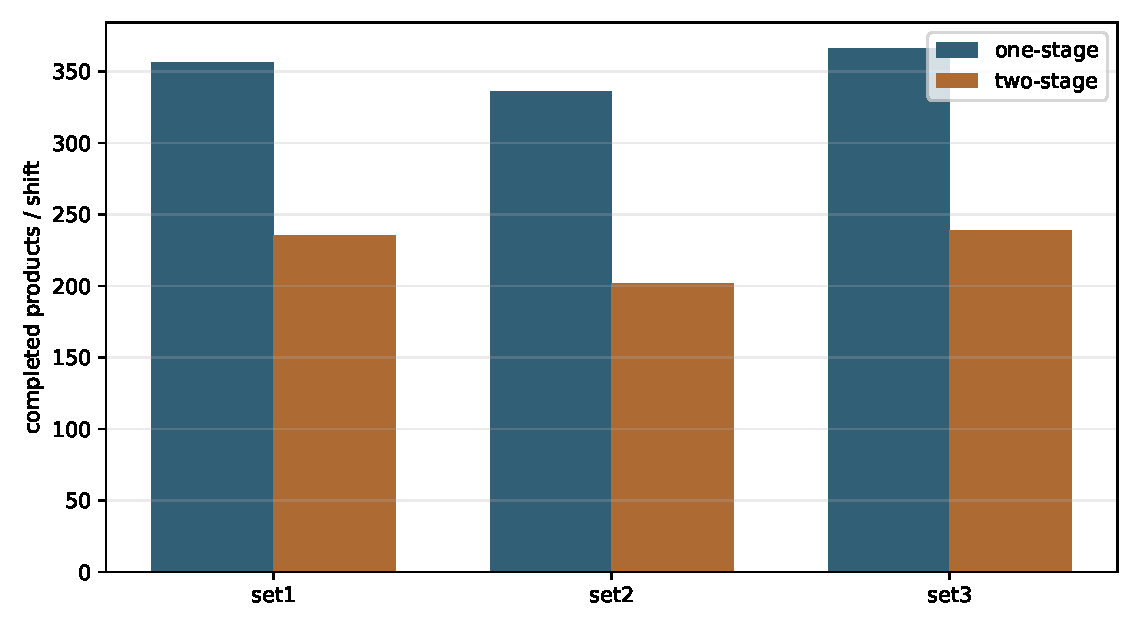
\includegraphics[width=0.82\textwidth]{figures/throughput.pdf}
\caption{三组参数下一道与两道工序的确定性班产量}
\label{fig:throughput-b}
\end{figure}

\subsection{成品间隔比单个平均数更能说明节奏}

一道工序三组数据在启动后的平均相邻成品间隔分别为 79.10、83.40 和 77.04 s，标准差分别为 42.88、29.84 和 39.13 s。间隔不是固定节拍，因为 RGV 会连续服务同一工位附近的多台 CNC，随后再跨工位处理另一批请求。图\ref{fig:intervals-b}保留了这种成组完成的离散结构。

\begin{table}[H]
\centering
\caption{一道工序成品时间接口}
\label{tab:one-stage-interval-b}
\small
\begin{tabular}{crrrrr}
\toprule
参数组 & 首件时刻/s & 末件时刻/s & 平均间隔/s & 间隔标准差/s & 最大间隔/s\\
\midrule
第1组 & 687 & 28768 & 79.10 & 42.88 & 191\\
第2组 & 729 & 28667 & 83.40 & 29.84 & 160\\
第3组 & 670 & 28791 & 77.04 & 39.13 & 180\\
\bottomrule
\end{tabular}
\end{table}

\begin{figure}[H]
\centering
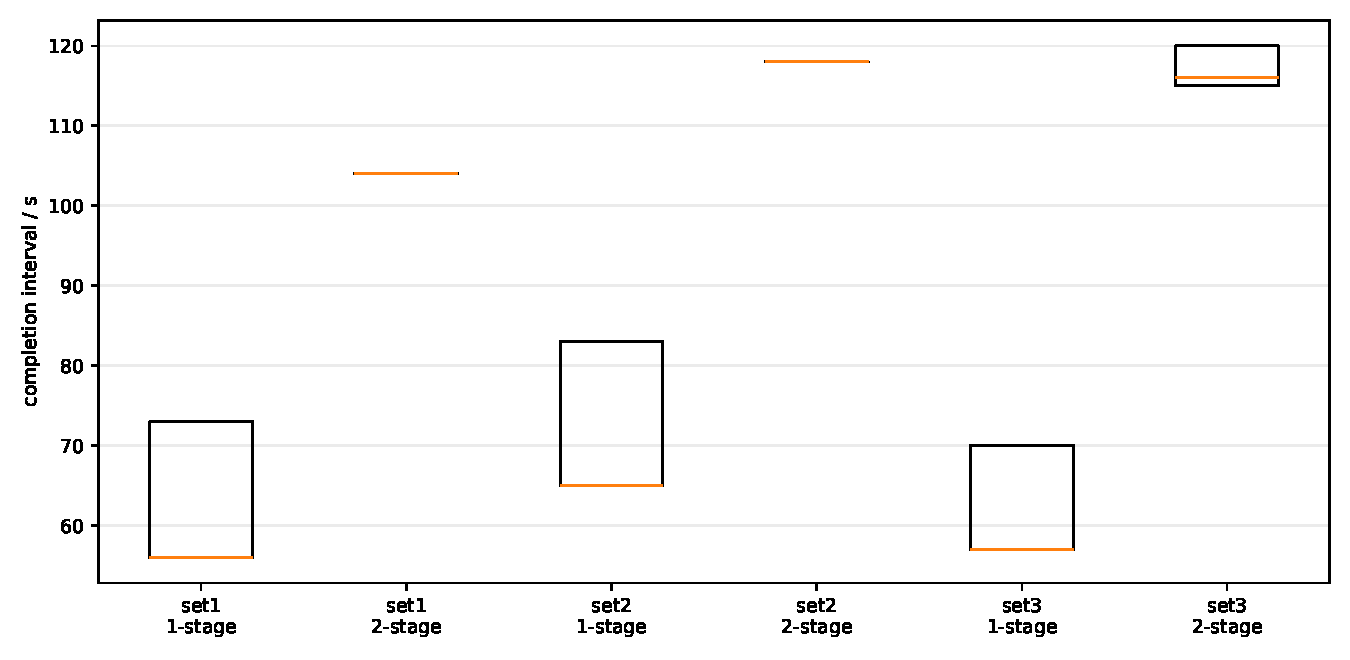
\includegraphics[width=0.86\textwidth]{figures/completion_intervals.pdf}
\caption{六种确定性情形在启动后的相邻成品间隔}
\label{fig:intervals-b}
\end{figure}

第1组日志有 365 次 RGV 服务，其中 8 次为首轮上料，357 次为卸下成品并装入新料；最终计入 356 件，是因为最后一个清洗动作越过班次截止。第2组对应 345 次服务和 336 件成品，第3组有 374 次服务和 366 件成品。动作数与成品数相差的原因可以从启动和截止两端解释，不需要在正文中用“取整误差”掩盖。

\subsection{加工松弛上界用于查错，不用于宣称最优}

暂时忽略 RGV 移动、上下料和清洗，只保留八台 CNC 的加工时间，可以得到一道工序的连续松弛上界
\begin{equation}
U_1=\frac{8H}{T_1}.
\label{eq:one-stage-bound-b}
\end{equation}
三组上界分别为 411.43、397.24 和 422.75 件，实际产量达到其 86.53\%、84.58\% 和 86.58\%。该比例不是通常意义上的最优性间隙，因为上界删除了 RGV 资源约束；它的用途是做数量级检查。若仿真产量超过 $U_1$，必有加工计时或完成计数错误。

\label{mcm-q2-end}

\section{任务二（二）模型的建立与求解：两道工序调度}
\label{mcm-q3-start}

\subsection{刀具分配先决定物料流向}

令
\begin{equation}
z_i=\begin{cases}
1,&\text{CNC $i$ 安装第一工序刀具},\\
2,&\text{CNC $i$ 安装第二工序刀具}.
\end{cases}
\label{eq:stage-allocation-b}
\end{equation}
为避免某道工序只有一台机器造成明显退化，又保留对不平衡加工时间的适应，枚举约束取为
\begin{equation}
2\leq \sum_{i=1}^{8}\mathbf 1_{\{z_i=1\}}\leq6.
\label{eq:allocation-range-b}
\end{equation}
对应的分配数为
\begin{equation}
\sum_{k=2}^{6}\binom{8}{k}=238.
\label{eq:allocation-count-b}
\end{equation}
每种分配分别运行三条调度规则，所以每组参数有 714 个“分配--规则”候选。第1工序机器数为 2、3、4、5、6 时，对应的候选对数为 84、168、210、168、84。

加工时间比可给出初始判断。若不计 RGV，平衡条件近似为
\begin{equation}
\frac{n_1}{T_{\mathrm{first}}}\approx \frac{8-n_1}{T_{\mathrm{second}}}.
\label{eq:stage-balance-b}
\end{equation}
第1、2组由此倾向 4/4 分配；第3组第二工序明显更快，倾向增加第一工序机器。枚举结果确实选择 5 台第一工序机，但具体是哪 5 台仍由工位位置和调度规则决定，不能只凭式\eqref{eq:stage-balance-b}确定。

\subsection{携带状态改变候选集合}

当 $b(t)=1$ 时，RGV 已携带半成品，只能寻找空闲或已完成的第二工序机：
\begin{equation}
\mathcal E_2^{(1)}(t)=\{i:z_i=2,\ s_i(t)\in\{\mathrm{empty},\mathrm{done}\}\}.
\label{eq:eligible-carry-b}
\end{equation}
若第二工序机已经完成，RGV 一次服务先卸出最终成品，再把携带的半成品装入；CNC 从服务结束开始加工，RGV随后清洗最终成品。这里不能先清洗再上料，否则会无故延迟第二工序。

当 $b(t)=0$ 时，候选既包括已完成或空闲的第一工序机，也包括需要单独卸出最终成品的第二工序机：
\begin{equation}
\mathcal E_2^{(0)}(t)=
\{i:z_i=1,\ s_i\in\{\mathrm{empty},\mathrm{done}\}\}
\cup\{i:z_i=2,\ s_i=\mathrm{done}\}.
\label{eq:eligible-free-b}
\end{equation}
访问完成的第一工序机后，RGV 同时为它装入新原料，并把卸下的半成品带走，故 $b$ 由 0 变为 1。访问仅有成品等待的第二工序机后，RGV 卸料并清洗，该机变为空闲，$b$ 仍为 0。

\begin{table}[H]
\centering
\caption{两道工序中的四类服务动作}
\label{tab:two-stage-actions-b}
\small
\begin{tabularx}{\textwidth}{p{3.5cm}p{3.2cm}p{4.2cm}X}
\toprule
动作 & 服务前状态 & 服务后的 CNC 与 RGV 状态 & 是否清洗\\
\midrule
第一工序首轮上料 & $z_i=1,s_i=empty,b=0$ & CNC加工，$b=0$ & 否\\
第一工序换料 & $z_i=1,s_i=done,b=0$ & CNC加工，$b=1$ & 否，卸出的是半成品\\
第二工序首轮上料 & $z_i=2,s_i=empty,b=1$ & CNC加工，$b=0$ & 否\\
第二工序换料 & $z_i=2,s_i=done,b=1$ & CNC加工，$b=0$ & 是，清洗卸出的成品\\
第二工序单独卸料 & $z_i=2,s_i=done,b=0$ & CNC空闲，$b=0$ & 是\\
\bottomrule
\end{tabularx}
\end{table}

\subsection{搜索结果先看分配，再看规则}

第1组的第一、第二工序时间接近，最优分配为 $12121212$，即奇数 CNC 做第一工序、偶数 CNC 做第二工序。这样的交错分配使 RGV 从任一第一工序机出发，都能在同一工位或相邻工位找到第二工序机。就近、预计完成和平衡规则的最高产量均为 235 件；本文在同值候选中保留就近规则。

第2组第一工序 280 s、第二工序 500 s，第二工序成为较慢的一侧。最优分配 $21211212$ 仍是 4/4，但第二工序机的位置不再严格奇偶交错。三条规则最高都达到 202 件，不过候选分布不同：就近规则的中位数为 151 件，平衡规则为 156 件。最终结果同值，不代表错误分配下的表现相同。

第3组第一工序 455 s、第二工序 182 s。若沿用 4/4，第二工序能力会大量空置；枚举选择 $21112121$，即第一工序由 CNC2、3、4、6、8 承担，第二工序由 CNC1、5、7 承担。预计服务完成优先得到 239 件，而就近和平衡规则均为 229 件。这里策略差异已经进入最终产量，所以不能再以实现简单为由保留就近规则。

\begin{table}[H]
\centering
\caption{两道工序的最终刀具分配与调度结果}
\label{tab:two-stage-results-b}
\scriptsize
\begin{tabularx}{\textwidth}{p{0.7cm}p{1.6cm}X p{1.5cm}rrrr}
\toprule
组 & 分配串 & 第一/第二工序 CNC & 规则 & 产量 & RGV忙 & RGV等 & CNC利用率\\
\midrule
1 & 12121212 & 1,3,5,7 / 2,4,6,8 & 就近 & 235 & 0.9221 & 0.0779 & 0.8174\\
2 & 21211212 & 2,4,5,7 / 1,3,6,8 & 就近 & 202 & 0.9216 & 0.0784 & 0.7035\\
3 & 21112121 & 2,3,4,6,8 / 1,5,7 & 预计完成 & 239 & 0.9903 & 0.0097 & 0.6789\\
\bottomrule
\end{tabularx}
\end{table}

\begin{figure}[H]
\centering
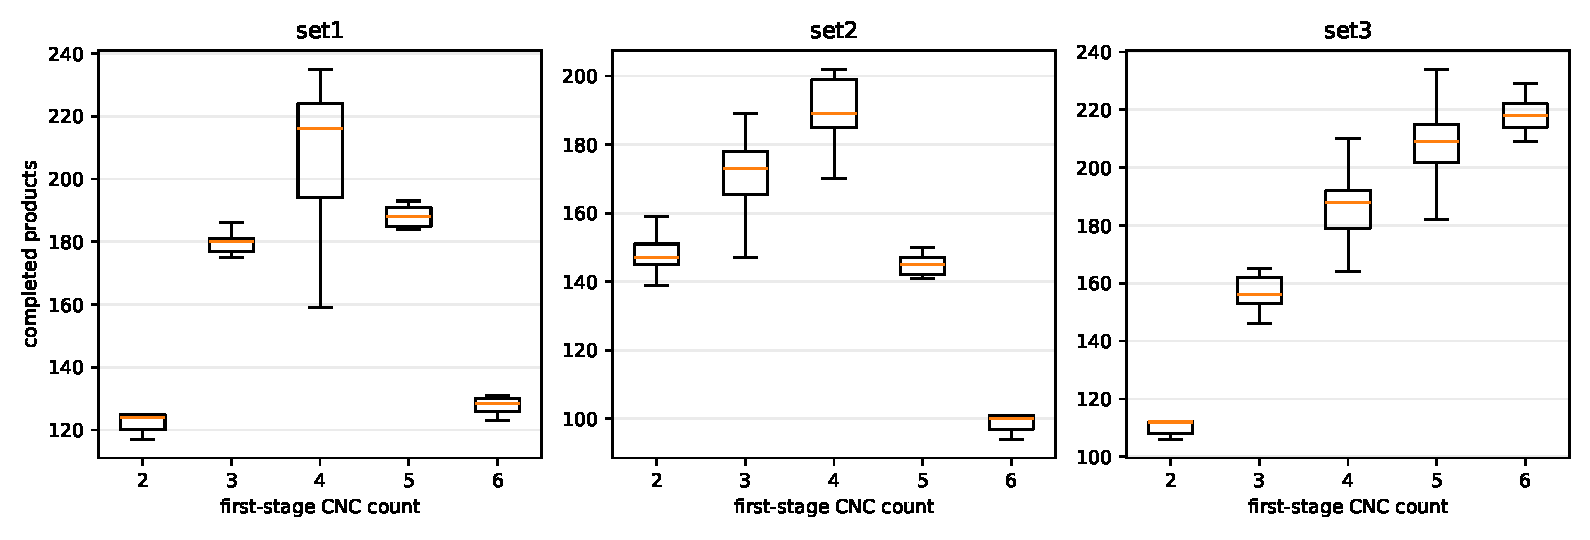
\includegraphics[width=0.94\textwidth]{figures/allocation_landscape.pdf}
\caption{不同第一工序 CNC 数量下的两道工序候选产量分布}
\label{fig:allocation-landscape-b}
\end{figure}

图\ref{fig:allocation-landscape-b}给出的不是一条光滑目标曲线。相同机器数下，不同工位组合会使产量跨越较大范围；同一分配换一条规则，也可能改变访问次序。第3组在 5 台第一工序机附近出现较高候选，与加工时间比一致，但只有特定分配和预计完成规则达到 239 件。因而“先确定台数、再任选位置”的简化不被结果支持。

\subsection{候选总体分布揭示规则的适用边界}

\begin{table}[H]
\centering
\caption{两道工序每条规则在 238 种分配上的产量统计}
\label{tab:policy-candidates-b}
\small
\begin{tabular}{clrrrrr}
\toprule
组 & 规则 & 最优 & 中位数 & 下四分位 & 上四分位 & 最优并列数\\
\midrule
1 & 平衡 & 235 & 184 & 175 & 193.00 & 8\\
1 & 预计完成 & 235 & 184 & 175 & 191.00 & 4\\
1 & 就近 & 235 & 184 & 175 & 193.75 & 8\\
2 & 平衡 & 202 & 156 & 145 & 185.00 & 4\\
2 & 预计完成 & 202 & 152 & 145 & 182.00 & 2\\
2 & 就近 & 202 & 151 & 145 & 179.00 & 4\\
3 & 平衡 & 229 & 188 & 156 & 208.00 & 1\\
3 & 预计完成 & 239 & 189 & 156 & 209.00 & 1\\
3 & 就近 & 229 & 180 & 156 & 208.00 & 1\\
\bottomrule
\end{tabular}
\end{table}

第2组平衡规则的中位数和上四分位数高于另外两条规则，但三者最高值相同。若研究目标是“在刀具分配暂时不能精确优化时选择一条较稳妥的规则”，平衡规则值得保留；若刀具分配已经枚举，最高产量处可选择更简单的就近规则。两个判断对应不同的实施条件，不能由同一张最优值表替代。

第3组则不同。预计完成规则不仅中位数略高，还把最优值从 229 提到 239。第二工序很短时，RGV 到达与服务结束的时间会直接决定一台第二工序机能否连续接料；只比较当前位置距离，会在局部近路上节省几十秒，却可能造成第一工序半成品在手中等待更久。

\begin{figure}[H]
\centering
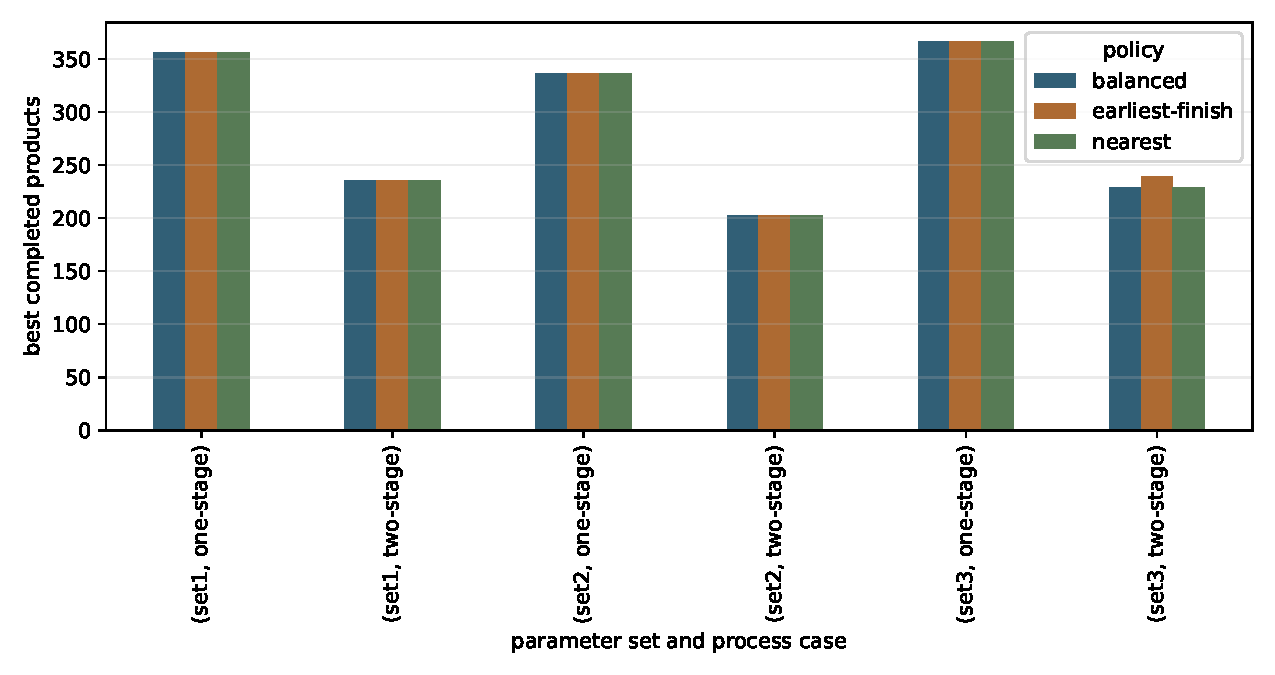
\includegraphics[width=0.90\textwidth]{figures/policy_comparison.pdf}
\caption{三种规则在各参数组和工序情形下的最高产量}
\label{fig:policy-comparison-b}
\end{figure}

\subsection{首小时动作图检查物料是否逆流}

图\ref{fig:first-hour-b}显示第1组两道工序前 3600 s 的 RGV 服务区间。首轮只有 4 台第一工序机接收原料；随后每次第一工序换料产生一个半成品，下一次涉及携带物料的服务只能落到第二工序机。图中服务块不是 CNC 的完整加工区间，而是 RGV 占用的移动、等待、上下料和清洗时间，故不能把空白解释成设备停机。

\begin{figure}[H]
\centering
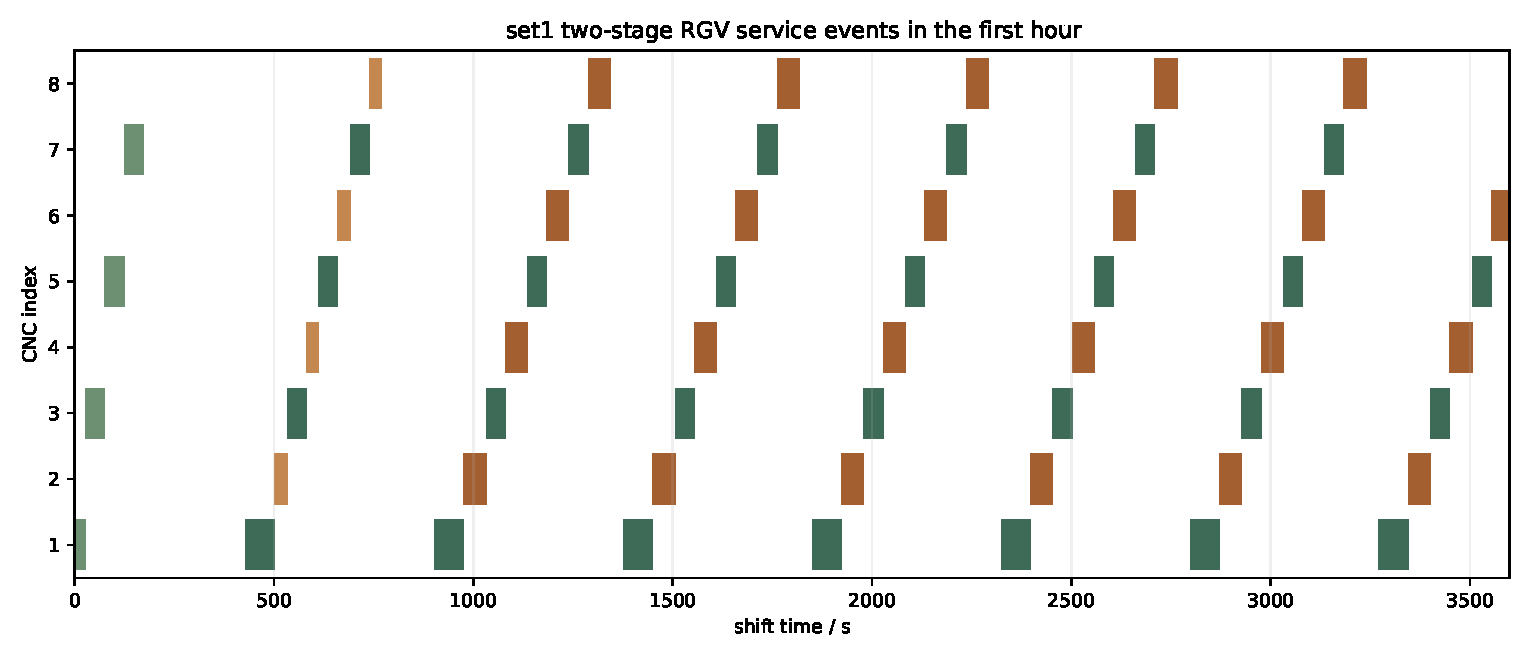
\includegraphics[width=0.94\textwidth]{figures/schedule_first_hour.pdf}
\caption{第1组两道工序首小时的 RGV 服务事件}
\label{fig:first-hour-b}
\end{figure}

第1组完整日志含 484 次服务：第一工序首轮上料 4 次、第二工序首轮上料 4 次、第一工序换料 240 次、第二工序换料 236 次。计入成品 235 件，仍有一次换料后的清洗跨越班次边界。第2组对应 417 次服务并完成 202 件；第3组除了 236 次第二工序换料，还出现 3 次“只卸成品”的动作，这说明某些时刻 RGV 没有携带半成品，却需要先释放已经完成的第二工序机。

\begin{table}[H]
\centering
\caption{两道工序动作日志的闭合计数}
\label{tab:action-count-b}
\small
\begin{tabular}{crrrrrr}
\toprule
组 & 第一工序首上料 & 第二工序首上料 & 第一工序换料 & 第二工序换料 & 第二工序单卸 & 成品\\
\midrule
1 & 4 & 4 & 240 & 236 & 0 & 235\\
2 & 4 & 4 & 207 & 202 & 0 & 202\\
3 & 5 & 6 & 242 & 236 & 3 & 239\\
\bottomrule
\end{tabular}
\end{table}

第3组第二工序首上料为 6 次，而分配中只有 3 台第二工序机，是因为日志动作名表示“向空闲第二工序机装入半成品”，其中有机器在单独卸出成品变空后再次执行该动作。动作计数按状态变化解释，不能简单把名称等同于班次初始上料。

\subsection{两工序松弛上界和瓶颈位置}

对固定分配，忽略 RGV 后的加工能力上界为
\begin{equation}
U_2=\min\left(\frac{n_1H}{T_{\mathrm{first}}},
\frac{n_2H}{T_{\mathrm{second}}}\right).
\label{eq:two-stage-bound-b}
\end{equation}
三组最终分配对应 $U_2=288.00,230.40,316.48$ 件，实际达到 81.60\%、87.67\%、75.52\%。第3组虽然班产量最高，但相对加工上界的比例最低；其 RGV 忙碌占比又达到 99.03\%，二者共同指出瓶颈已从单台 CNC 加工转到 RGV 的跨工序转运。

\label{mcm-q3-end}

\section{任务二（三）模型的建立与求解：故障情景}
\label{mcm-q4-start}

\subsection{故障发生在加工开始之后}

每次 CNC 开始加工时独立生成 $U\sim\mathrm{Uniform}(0,1)$。若 $U<0.01$，本次加工被标记为故障；故障发生到加工开始后的时间和修复时间分别取
\begin{equation}
T_f\sim\mathrm{Uniform}(0,T_i),\qquad
T_r\sim\mathrm{Uniform}(600,1200).
\label{eq:failure-model-b}
\end{equation}
该 CNC 在 $T_f+T_r$ 内不可服务，未完成物料报废，修复结束后状态变为空闲。这里没有把故障修复时间加在原加工完成时刻之后，而是从实际故障点开始计算；也没有让 RGV 在故障点额外执行未由题面给出的搬运。

故障概率按“加工启动次数”而不是按秒解释。若按每秒 1\% 触发，几乎所有长加工都会故障；若固定每班只有 1\% 的机器故障，又会低估加工次数较多的参数组。题面只给出约 1\%，本文采用上述可复算解释，并把它列入结论边界。

\subsection{随机协议在看结果以前固定}

每个参数组、每种工序情形独立运行 200 次，随机种子从 20180915 按参数组和运行编号确定。每次运行沿用确定性情形已经选定的刀具分配和调度规则，不在故障发生以后重新搜索一套更有利的规则。这样比较的是同一策略从无故障到故障情景的产量损失。

每次运行记录班产量、报废数和故障数。对班产量 $N_1,\ldots,N_{200}$，报告
\begin{equation}
\bar N=\frac1{200}\sum_{j=1}^{200}N_j,qquad
s_N=\sqrt{\frac1{199}\sum_{j=1}^{200}(N_j-\bar N)^2},
\label{eq:mc-summary-b}
\end{equation}
并给出 5\%、50\%、95\% 分位数。200 次只能描述本次情景抽样，不能把尾部分位数解释成严格可靠性保证。

\begin{table}[H]
\centering
\caption{1\% 故障情景下的 200 次班产量统计}
\label{tab:failure-results-b}
\small
\begin{tabular}{ccrrrrr}
\toprule
组 & 工序 & 均值 & 标准差 & 5\%分位 & 中位数 & 95\%分位\\
\midrule
1 & 一道 & 350.595 & 3.921 & 343.00 & 351 & 356.00\\
1 & 两道 & 228.390 & 5.600 & 218.00 & 229 & 236.05\\
2 & 一道 & 330.385 & 5.427 & 322.00 & 331 & 338.00\\
2 & 两道 & 189.765 & 5.328 & 180.95 & 190 & 199.00\\
3 & 一道 & 359.850 & 4.675 & 352.00 & 361 & 366.05\\
3 & 两道 & 220.990 & 7.903 & 209.00 & 221 & 234.00\\
\bottomrule
\end{tabular}
\end{table}

图\ref{fig:failure-distribution-b}显示一道工序的分布较集中，两道工序尤其是第3组向低产量一侧展开。第3组确定性策略把 RGV 使用率推到 99\% 以上，故障造成的空档难以由剩余路线吸收；同时 5 台第一工序机中的任一停机会改变半成品供应节奏。较快的第二工序本身不能消除这种上游依赖。

\begin{figure}[H]
\centering
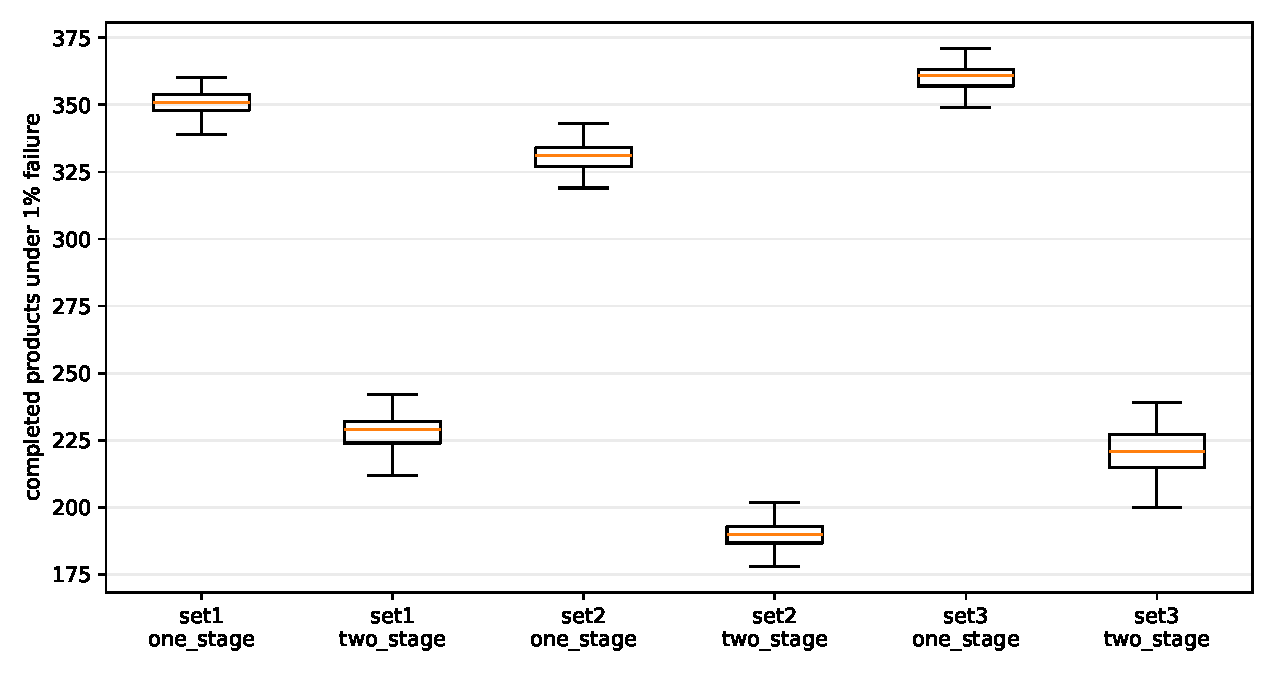
\includegraphics[width=0.88\textwidth]{figures/failure_distribution.pdf}
\caption{1\% 故障情景下六种情形的班产量分布}
\label{fig:failure-distribution-b}
\end{figure}

\subsection{损失相对无故障基线解释}

将每次故障运行的产量与同参数、同策略的确定性产量作差，可以避免把三组本来不同的加工速度混在一起。第1、2、3组一道工序的平均损失为 5.405、5.615、6.150 件；两道工序分别损失 6.610、12.235、18.010 件。

\begin{table}[H]
\centering
\caption{故障损失及保持确定性产量 95\% 的比例}
\label{tab:failure-loss-b}
\small
\begin{tabular}{ccrrrrr}
\toprule
组 & 工序 & 平均损失 & 损失中位数 & 损失95\%分位 & 最大损失 & 达到基线95\%比例\\
\midrule
1 & 一道 & 5.405 & 5 & 13.00 & 17 & 1.000\\
1 & 两道 & 6.610 & 6 & 17.00 & 23 & 0.775\\
2 & 一道 & 5.615 & 5 & 14.00 & 33 & 0.965\\
2 & 两道 & 12.235 & 12 & 21.05 & 26 & 0.310\\
3 & 一道 & 6.150 & 5 & 14.00 & 25 & 0.990\\
3 & 两道 & 18.010 & 18 & 30.00 & 39 & 0.250\\
\bottomrule
\end{tabular}
\end{table}

\begin{figure}[H]
\centering
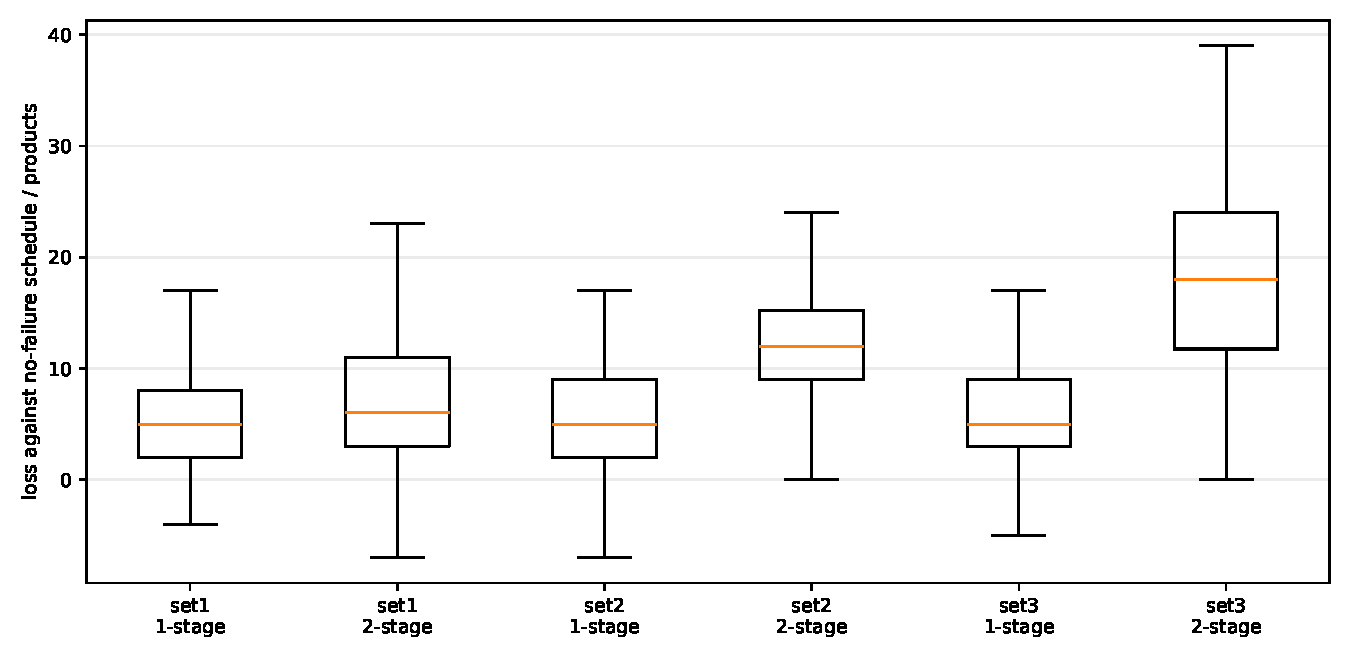
\includegraphics[width=0.88\textwidth]{figures/failure_loss.pdf}
\caption{故障运行相对同策略无故障班产量的损失}
\label{fig:failure-loss-b}
\end{figure}

“达到基线 95\% 的比例”只描述本次 200 次运行。第3组两道工序仅有 25\% 运行达到该阈值，不能据此推出真实工厂恰有 75\% 班次不达标，因为故障独立性、发生时刻分布和修复时间分布都是题面之外的情景设定。它可以支持的判断是：在同一随机协议下，该方案对故障的产量损失比一道工序和第1组两道工序更明显。

\subsection{报废数不等于产量损失}

六种情形的平均报废数依次为 3.600、4.725、3.380、3.960、3.570、4.505 件，而平均产量损失有时远高于报废数。原因是故障除了报废当前物料，还占用 CNC 的修复时间，并改变 RGV 后续访问；两道工序中还会造成半成品供应或第二工序空闲。因此不能用“平均报废 4.5 件”直接替代“平均少完成 18.01 件”。

这个差值提供了一个公开判断入口。若某次仿真损失与报废数完全相等，应检查修复时长是否真的进入事件时钟；若损失远大于报废数，则要回看停机发生在哪一道工序、是否打断了携带半成品后的候选集合，而不是把额外损失统称为随机波动。

\label{mcm-q4-end}

\section{数值求解实现与代表性事件复盘}

\subsection{事件循环没有人为时间步长}

本题给出的移动、上下料和加工时间均为整数秒，但模型没有按 1 s 或更细网格扫描。当前时刻若没有可服务 CNC，程序直接跳到最近的加工完成或维修结束时刻；选定目标以后，再依次加上移动、等待、上下料和清洗的实际持续时间。因此产量不存在由时间步长取整产生的误差，离散性来自动作本身和 8 h 截止边界。

一次事件循环按表\ref{tab:event-loop-b}执行。第三步先更新全部到期 CNC，再构造候选；若先构造候选后更新，恰在当前时刻完成的机器会被漏掉一个决策轮次。第七步在上下料结束时启动 CNC，第八步才处理最终成品清洗；二者的顺序对应前文的并发关系。

\begin{table}[H]
\centering
\caption{一个事件循环的实际执行顺序}
\label{tab:event-loop-b}
\small
\begin{tabularx}{\textwidth}{p{1.1cm}p{4.2cm}p{5.0cm}X}
\toprule
步序 & 读取的状态 & 执行动作 & 写出的状态或日志\\
\midrule
1 & 当前 $t,p,b$ 与八台 CNC & 检查是否达到班次边界 & 继续或停止\\
2 & 各 CNC 的 $s_i,r_i$ & 将到期加工更新为 done，将到期故障更新为 empty & 请求集、报废和故障累计\\
3 & 工序类型与 $b$ & 按式\eqref{eq:eligible-one-b}、\eqref{eq:eligible-carry-b}或\eqref{eq:eligible-free-b}构造候选 & $\mathcal E(t)$\\
4 & 空候选集 & 跳到最近 $r_i$ & RGV等待时间、新时刻\\
5 & 非空候选集 & 计算三类评分之一并取最小 & 目标 CNC\\
6 & 当前位置与目标位置 & 推进移动和必要等待 & RGV忙碌/等待、服务开始时刻\\
7 & 目标 CNC 状态 & 执行相应上下料并启动下一次加工 & $s_i,r_i,b$\\
8 & 是否卸出最终成品 & 推进清洗；若不晚于 $H$ 则计数 & 累计成品、动作起止和新位置\\
\bottomrule
\end{tabularx}
\end{table}

若最后一步跨过 $H$，程序保留动作日志的截断终点，但不把该成品计入班产量。忙碌和等待的累计也只取 $[0,H]$ 内的部分。这个处理让“产量截止”“动作日志截止”和“资源利用率截止”使用同一条边界。

\subsection{第1组两道工序的前十四次动作}

表\ref{tab:first-actions-b}从完整日志原样抽取前十四次服务。前四次把生料装入 CNC1、3、5、7；CNC1 在 $28+400=428$ s 完成第一工序。RGV 此时位于工位 3，返回工位 0 需要 46 s，再为 CNC1 换料 28 s，所以该动作从 428 s 延续到 502 s。随后 CNC2 与 CNC1 位于同一工位，只需 31 s 上料，半成品在 533 s 进入第二工序。

\begin{table}[H]
\centering
\caption{第1组两道工序开局动作日志}
\label{tab:first-actions-b}
\scriptsize
\begin{tabular}{rrrrp{5.8cm}r}
\toprule
起点/s & 终点/s & CNC & 工位 & 动作 & 累计成品\\
\midrule
0 & 28 & 1 & 0 & 第一工序首轮上料 & 0\\
28 & 76 & 3 & 1 & 移动并完成第一工序首轮上料 & 0\\
76 & 124 & 5 & 2 & 移动并完成第一工序首轮上料 & 0\\
124 & 172 & 7 & 3 & 移动并完成第一工序首轮上料 & 0\\
428 & 502 & 1 & 0 & 返回工位0，第一工序换料并携带半成品 & 0\\
502 & 533 & 2 & 0 & 向第二工序机装入半成品 & 0\\
533 & 581 & 3 & 1 & 第一工序换料并携带半成品 & 0\\
581 & 612 & 4 & 1 & 向第二工序机装入半成品 & 0\\
612 & 660 & 5 & 2 & 第一工序换料并携带半成品 & 0\\
660 & 691 & 6 & 2 & 向第二工序机装入半成品 & 0\\
691 & 739 & 7 & 3 & 第一工序换料并携带半成品 & 0\\
739 & 770 & 8 & 3 & 向第二工序机装入半成品 & 0\\
902 & 976 & 1 & 0 & 第一工序换料并携带半成品 & 0\\
976 & 1032 & 2 & 0 & 卸出首件成品、装入半成品并清洗 & 1\\
\bottomrule
\end{tabular}
\end{table}

从 770 s 到 902 s 没有可执行请求，RGV 原地等待；这段时间不是算法漏排。首件第二工序于 $533+378=911$ s 附近完成，但 RGV 在 902 s 已开始处理 CNC1 的第一工序成品，完成该动作后在同一工位访问 CNC2，最终于 1032 s 完成上下料和清洗。动作序列显示了一个局部取舍：先获取下一件半成品，再用同一工位的第二工序机完成“卸成品--装半成品”，少一次空驶。

这段复盘还说明日志中的 start 不是 CNC 加工完成时刻，而是 RGV 开始本次移动或服务的时刻；end 包含本次移动、等待、上下料以及必要清洗。若把 start/end 直接画成 CNC 加工甘特图，会把 RGV 占用和 CNC 占用混为一谈。图\ref{fig:first-hour-b}因此明确标为 RGV 服务事件。

\subsection{最优候选附近不是每组都同样平坦}

第1组存在多种 235 件分配，第2组也有多种 202 件分配；第3组的 239 件候选只有一个。表\ref{tab:best-neighborhood-b}列出最优附近的实际记录。前两组可以在同产量分配中进一步按刀具安装便利、维护或路线偏好选择，第3组若换到次优分配，当前规则下会立即减少 1--2 件。

\begin{table}[H]
\centering
\caption{两道工序最优候选附近的分配记录}
\label{tab:best-neighborhood-b}
\small
\begin{tabular}{cclrr}
\toprule
组 & 分配串 & 规则 & 班产量 & 与本组最优差\\
\midrule
1 & 12121212 & 就近 & 235 & 0\\
1 & 12121221 & 就近 & 235 & 0\\
1 & 12122112 & 平衡 & 235 & 0\\
2 & 21211212 & 就近 & 202 & 0\\
2 & 21212112 & 预计完成 & 202 & 0\\
2 & 12211212 & 平衡 & 200 & 2\\
3 & 21112121 & 预计完成 & 239 & 0\\
3 & 21112112 & 预计完成 & 238 & 1\\
3 & 12211121 & 预计完成 & 238 & 1\\
3 & 12112121 & 预计完成 & 237 & 2\\
3 & 11212111 & 就近 & 229 & 10\\
\bottomrule
\end{tabular}
\end{table}

这里不使用“参数微调”描述分配变化。把一个字符从 1 改成 2 会改变某台 CNC 的刀具、两道工序的总能力和半成品可达位置，是离散结构切换。第3组从 $21112121$ 换成 $21112112$ 时，第一工序机器总数仍为 5，但 CNC7、8 的角色互换，班产量少 1 件；差异来自工位和奇偶上下料时间共同变化。

\subsection{运行规模和穷举边界}

一道工序每组只运行三条规则，共 9 个确定性候选。两道工序每组有 $238\times3=714$ 个候选，三组合计 2142 个；候选表共 2151 行。每次事件最多比较 8 台 CNC，调度日志的行数在 345--492 之间，因此确定性搜索的主要成本来自重复仿真，而不是单次候选评分。

故障阶段不再枚举刀具分配，而是对六个已选定方案各运行 200 次，共 1200 次。这样做的计算对象是“固定策略的故障表现”。若每个故障样本都重新枚举 238 种分配，得到的将是知道整班故障实现以后才作出的事后策略，不是可在班次开始前执行的方案。

程序固定随机种子只为复算同一批样本。固定种子不会让 200 次样本自动具有代表性，也不应把相同输出称为模型稳定；稳定性要看不同故障实现下的分布和方案排序，而不是同一随机序列能否重复打印。

\subsection{极端故障运行用于检查损失传播}

表\ref{tab:worst-failure-b}列出每种情形在 200 次运行中的最低班产量。第2组一道工序的最低值为 303 件，只发生 5 次故障，却比确定性基线少 33 件；故障次数不是最大，损失却最大，说明故障发生时刻和所占机器位置比单纯计数更重要。第3组两道工序最低完成 200 件，14 次故障对应 14 件报废，产量损失却达到 39 件。

\begin{table}[H]
\centering
\caption{每种情形的最低产量运行}
\label{tab:worst-failure-b}
\small
\begin{tabular}{ccrrrrr}
\toprule
组 & 工序 & 运行编号 & 最低产量 & 故障数 & 报废数 & 相对基线损失\\
\midrule
1 & 一道 & 160 & 339 & 8 & 8 & 17\\
1 & 两道 & 176 & 212 & 9 & 9 & 23\\
2 & 一道 & 126 & 303 & 5 & 5 & 33\\
2 & 两道 & 9 & 176 & 7 & 7 & 26\\
3 & 一道 & 190 & 341 & 13 & 13 & 25\\
3 & 两道 & 190 & 200 & 14 & 14 & 39\\
\bottomrule
\end{tabular}
\end{table}

最低值只是一条样本轨迹，不能替代 5\% 分位数。保留它的原因是可用于查错：若最低运行的损失小于报废数，完成计数或报废计数可能不一致；若少量故障造成较大损失，则应回放这些故障落在哪些 CNC 和工序，而不是删除所谓离群点。当前结果满足损失不小于报废数，且两道工序的极端损失与携带和工序供应链相符。

\section{结果分析、模型检验与跨情形复核}

\subsection{资源时间在班次边界内闭合}

RGV 忙碌时间包括移动、上下料和清洗，等待时间包括没有可执行请求或到达后等待 CNC 完成。两者均截断到 $H$，故确定性运行应满足
\begin{equation}
T_{\mathrm{busy}}+T_{\mathrm{wait}}=H.
\label{eq:time-closure-b}
\end{equation}
六种情形的占比之和均为 1。初版诊断曾出现略大于 1 的结果，追查后发现最后一次动作跨越班次边界时仍被完整计入资源时间；修正只改变利用率，不改变按清洗完成时刻判定的班产量。

\begin{figure}[H]
\centering
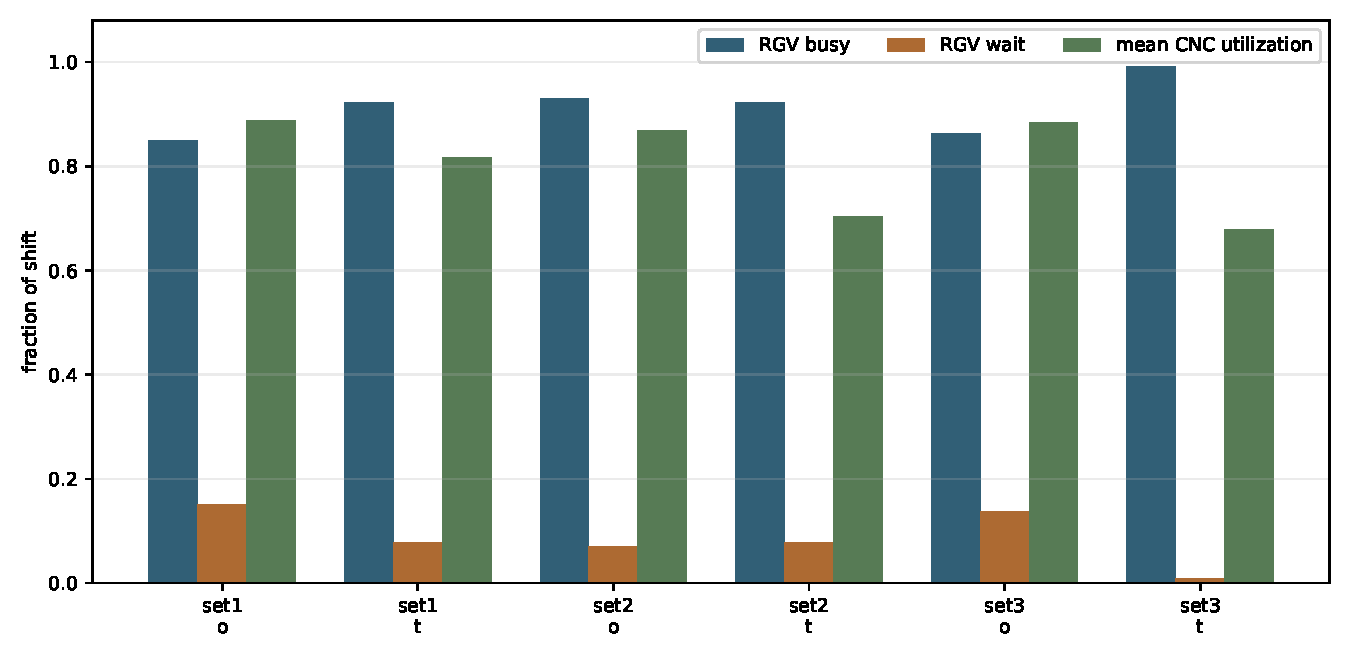
\includegraphics[width=0.90\textwidth]{figures/resource_utilization.pdf}
\caption{RGV 忙碌、等待与平均 CNC 利用率}
\label{fig:resource-utilization-b}
\end{figure}

第3组两道工序的 RGV 忙碌占比为 0.9903，平均 CNC 利用率却只有 0.6789。二者同时出现并非矛盾：RGV 几乎一直在转运和服务，但 5/3 的工序分配使部分第二工序机等待半成品，第一工序机也可能等待 RGV 卸料。继续增加某类 CNC 不能消除单辆 RGV 的串行约束。

\subsection{加工能力上界与实际结果对照}

\begin{table}[H]
\centering
\caption{忽略 RGV 后的加工松弛上界}
\label{tab:capacity-bound-b}
\small
\begin{tabular}{ccrrrr}
\toprule
组 & 工序 & 第一/第二工序机数 & 松弛上界/件 & 实际/件 & 实际/上界\\
\midrule
1 & 一道 & 8/0 & 411.43 & 356 & 0.8653\\
1 & 两道 & 4/4 & 288.00 & 235 & 0.8160\\
2 & 一道 & 8/0 & 397.24 & 336 & 0.8458\\
2 & 两道 & 4/4 & 230.40 & 202 & 0.8767\\
3 & 一道 & 8/0 & 422.75 & 366 & 0.8658\\
3 & 两道 & 5/3 & 316.48 & 239 & 0.7552\\
\bottomrule
\end{tabular}
\end{table}

第2组两道工序达到上界的比例最高，并不意味着它的绝对产量最高。第二工序 500 s 使加工上界本身只有 230.4 件，RGV 的额外损失空间较小；第3组的上界高，但短第二工序要求更频繁的转运，RGV 约束删除后留下的上界较松。上界用于查错和定位瓶颈，不能单独评价方案优劣。

\subsection{动作计数检验物料守恒}

两道工序中，每个计入的成品必须对应一次第二工序最终卸料；每个装入第二工序的半成品必须来自此前一次第一工序卸料。班次末允许存在已经完成第一工序但尚未完成第二工序的在制品，所以两类累计数不要求严格相等，但必须满足
\begin{equation}
N_{\mathrm{final}}\leq N_{\mathrm{stage1\ unload}},\qquad
N_{\mathrm{stage2\ load}}\leq N_{\mathrm{stage1\ unload}}.
\label{eq:material-invariant-b}
\end{equation}
诊断文件还检查累计成品计数单调不减，六份调度日志的末值与汇总 JSON 一致。上述检查可以发现半成品被重复装入或成品在未清洗时计数，却不能证明当前候选规则已经最优。

\begin{table}[H]
\centering
\caption{本次实现的状态与结果检查}
\label{tab:invariants-b}
\small
\begin{tabularx}{\textwidth}{p{4.0cm}p{4.5cm}X}
\toprule
检查 & 当前结果 & 不能由此推出的结论\\
\midrule
RGV 忙碌加等待等于 8 h & 六种确定性情形均闭合 & 不证明动作次序最优\\
累计成品数单调不减 & 六份日志全部通过 & 不证明没有漏记在制品\\
日志末值等于汇总结果 & 356/235、336/202、366/239 均一致 & 不证明题面之外参数正确\\
两工序物料不逆流 & 第二工序装料均由携带状态触发 & 不证明刀具分配全局最优\\
产量不超过加工松弛上界 & 六种情形均低于上界 & 上界删除了 RGV 约束，间隙不等于最优性间隙\\
\bottomrule
\end{tabularx}
\end{table}

\subsection{结果文件与正文采用单向接口}

求解器生成 2151 行候选表、1200 行故障运行表和 6 份调度日志；诊断脚本读取这些文件，生成策略统计、动作闭合、加工上界和故障损失，再由正文选取对应字段。正文不重新模拟一遍调度，也不从图上反读数字。

\begin{table}[H]
\centering
\caption{结果制品及其正文职责}
\label{tab:result-interface-b}
\small
\begin{tabularx}{\textwidth}{p{4.1cm}p{4.4cm}X}
\toprule
制品 & 主要字段 & 正文使用位置\\
\midrule
\path{summary.json} & 六种确定性结果、故障均值和分位数 & 表\ref{tab:one-stage-results-b}、\ref{tab:two-stage-results-b}、\ref{tab:failure-results-b}\\
\path{strategy_candidates.csv} & 分配、规则、班产量 & 表\ref{tab:policy-candidates-b}和图\ref{fig:allocation-landscape-b}\\
\path{schedule_*.csv} & 动作起止、CNC、累计成品 & 表\ref{tab:action-count-b}和图\ref{fig:first-hour-b}\\
\path{failure_runs.csv} & 每次班产量、报废、故障数 & 图\ref{fig:failure-distribution-b}、\ref{fig:failure-loss-b}\\
\path{diagnostics.json} & 闭合检查、间隔、上界和损失 & 表\ref{tab:capacity-bound-b}、\ref{tab:invariants-b}\\
\path{model_pipeline.py} & 状态更新、枚举和随机仿真 & 全部原始结果\\
\path{diagnostics.py} & 独立汇总与绘图 & 结果解释和复核\\
\bottomrule
\end{tabularx}
\end{table}

若修改清洗并发关系，受影响的不只是资源利用率；CNC 重启时刻、RGV 下一可用时刻、候选访问序列、班产量和故障运行都会改变。因此正式复算必须先重跑主求解器，再运行诊断脚本和正文同步审计，不能只替换表格中的一个产量数字。

\section{灵敏度与稳健性：改变的是参数还是事件顺序}

\subsection{三组参数本身构成结构扰动}

三组数据同时改变移动、加工、上下料和清洗时间，不是单变量灵敏度试验。它们仍提供两个稳定信号：一道工序三条规则均同值，而两道工序第3组出现规则分化；前者说明同质长加工下局部规则差异被设备并行吸收，后者说明工序时间严重不平衡时，访问完成时刻进入了关键决策。

第1、2组两道工序都选 4/4，第3组选 5/3，说明刀具数量没有被固定模板锁死。更重要的是，第3组不是只把一台 CNC 从第二工序改成第一工序，工位组合也随搜索改变。若只对 $n_1$ 做连续比例分析，无法识别同一台数下不同位置造成的产量分散。

\subsection{规则权重只作对照，不作精确标定}

平衡评分中的 0.8 和 0.35 没有来自现场数据，本文不围绕小数末位做伪精细调参。它的作用是提供一条介于就近和预计完成之间的候选：若它在三个参数组均显著优于两条基线，再值得建立权重搜索；当前结果中第1、2组最优值并未提高，第3组还低于预计完成，因此没有继续扩展权重维度。

这个取舍保留了比较过程，但没有把每一问写成相同的“基线不足--复杂模型改进”。第1、2组没有观察到复杂规则的最终产量收益，正式方案反而保留简单规则；第3组出现 10 件差距后，才更换为预计完成优先。模型复杂度由结果分叉决定，而不是预先规定。

\subsection{故障情景的结果边界}

若故障概率、故障时刻或修复时间分布改变，表\ref{tab:failure-results-b}必须全部重算。当前随机协议没有考虑同一刀具批次造成的相关故障，也没有考虑维修人员同时只能处理一台机器。因而 5\% 分位数只能用于比较六种情形在同一假设下的相对脆弱性，不能直接作为现场最低产量承诺。

\begin{table}[H]
\centering
\caption{关键设定的扰动方向和需重算对象}
\label{tab:sensitivity-contract-b}
\small
\begin{tabularx}{\textwidth}{p{3.7cm}p{4.5cm}X}
\toprule
改变的设定 & 首先改变的事件或约束 & 必须同步更新的输出\\
\midrule
清洗允许与移动并行 & RGV 下一可用时刻 & 全部调度日志、产量和利用率\\
故障概率 & 加工开始后的状态分支 & 1200 行故障运行和分位数\\
修复时间分布 & CNC 重新进入候选集的时刻 & 故障损失与策略访问序列\\
第一工序机数量范围 & 分配枚举集合 & 候选总数和最优性边界\\
平衡规则权重 & 每个决策时刻的候选排序 & 候选表；确定性和故障基线\\
班次长度 & 截止动作和启动期占比 & 班产量、末件时刻和资源闭合\\
\bottomrule
\end{tabularx}
\end{table}

\section{可执行调度策略汇总}

\subsection{班次开始前确定的量}

一道工序不需要刀具分配，八台 CNC 全部安装同一刀具。两道工序在班次开始前按表\ref{tab:operating-plan-b}安装刀具，班次中不更换。随机故障情形沿用相同配置和规则，不根据已经发生的整班故障记录事后更换方案。这样，确定性和故障结果具有同一实施基线。

\begin{table}[H]
\centering
\caption{六种确定性工况的现场执行方案}
\label{tab:operating-plan-b}
\small
\begin{tabularx}{\textwidth}{p{1.3cm}p{2.1cm}p{3.4cm}p{3.0cm}X}
\toprule
组 & 工序 & 刀具配置 & 在线规则 & 每次完成动作后的判断\\
\midrule
1 & 一道 & 八台同刀具 & 就近优先 & 从空闲或完成 CNC 中取移动加等待最小者\\
2 & 一道 & 八台同刀具 & 就近优先 & 同上，奇偶上下料时间按本组参数读取\\
3 & 一道 & 八台同刀具 & 就近优先 & 同上，不因加工较快而预设固定循环\\
1 & 两道 & 1,3,5,7 为第一工序 & 就近优先 & 携带半成品时只访问第二工序机\\
2 & 两道 & 2,4,5,7 为第一工序 & 就近优先 & 无半成品时可先卸出已完成的第二工序成品\\
3 & 两道 & 2,3,4,6,8 为第一工序 & 预计服务完成优先 & 比较到达、等待和上下料结束时刻\\
\bottomrule
\end{tabularx}
\end{table}

\subsection{班次中的共同操作规则}

每完成一次移动、上下料或清洗，控制器读取八台 CNC 的状态和预计完成时刻。若有可服务请求，按当前工况的评分选择目标；若没有请求，RGV 原地等待到最近事件。目标机上下料结束后立即发送开工指令。卸出的是最终成品时，RGV 在原位完成清洗再选择下一目标；卸出的是第一工序半成品时，RGV 不清洗，下一目标只能从第二工序机中选择。

CNC 故障后，该机从候选集中移除，当前物料计为报废；修复结束时状态恢复为空闲，并按所属工序重新请求物料。其他 CNC 和 RGV 不停机等待故障机，仍按当前候选集合运行。这个动作是动态调度对故障的实际响应，不需要在每次故障后重新枚举刀具配置。

\subsection{班次结束时提交的结果}

班次截止时输出成品总数、每次服务的起止时刻和 CNC 编号。正在加工、已完成但尚未卸下、或已经卸下但清洗跨过 28800 s 的物料不计入成品。确定性方案同时输出 RGV 忙碌/等待和平均 CNC 利用率；故障方案按 200 次运行输出班产量分布、报废数和相对确定性基线的损失。附件表若需要逐件记录，应直接从六份 \path{schedule_*.csv} 生成，不能根据平均间隔倒推虚构时刻。

\section{被排除的简化方案}

\subsection{不把清洗时间加到 CNC 加工时间}

双手爪上下料结束以后，新物料已在 CNC 上，题面清洗槽位于 RGV。把清洗时间并入 CNC 加工会使所有机器每件多等待 25--30 s，并错误地降低并行度。正确做法是 CNC 从上下料结束开工，RGV 在清洗结束以后才能移动。两个时钟在式\eqref{eq:cnc-restart-b}和式\eqref{eq:rgv-next-b}处分开。

\subsection{不让 RGV 在清洗时提前出发}

附件明确说明清洗过程中 RGV 不能移动。若把清洗看成独立后台设备，RGV 每完成一件便可提前 25--30 s 访问下一台 CNC，8 h 内会累计数百次不允许的重叠。这个简化会提高产量，却没有可执行的物理动作支撑。

\subsection{不把两道工序压成等效加工时间}

把 $T_{\mathrm{first}}+T_{\mathrm{second}}$ 当作一道工序时间，会删除刀具分配、半成品携带和第二工序等待三个核心约束。第3组的 $455+182$ s 看似只比一道工序的 545 s 稍长，但实际还要在两个 CNC 之间转运，且 RGV 忙碌占比接近 1。等效加工时间无法解释 5/3 分配和预计完成规则的 10 件收益。

\subsection{不以平均故障损失直接修改确定性产量}

用“确定性产量减平均故障数”只能处理报废，不能处理修复占用和访问序列变化。第3组两道工序平均报废约 4.505 件，平均产量损失却为 18.010 件，二者相差超过 13 件。蒙特卡洛不是为了制造随机图，而是为了保留故障发生位置对后续状态的传播。

\begin{table}[H]
\centering
\caption{替代简化、遗漏对象及其判定证据}
\label{tab:rejected-b}
\small
\begin{tabularx}{\textwidth}{p{3.4cm}p{4.2cm}p{4.5cm}X}
\toprule
简化 & 被删掉的对象 & 会出现的偏差 & 本文证据\\
\midrule
清洗并入加工 & CNC 与 RGV 的并发 & CNC 利用率偏低 & 双时钟状态更新\\
清洗后台执行 & RGV 串行动作 & 班产量偏高 & 资源时间闭合\\
固定循环路线 & 完成事件和当前位置 & 无法响应错开的请求 & 逐事件动作日志\\
连续比例后取整 & 工位组合 & 同台数候选差异被删除 & 图\ref{fig:allocation-landscape-b}\\
两工序等效成一道 & 携带状态和工序先后 & 物料可能逆流或重复 & 式\eqref{eq:eligible-carry-b}、\eqref{eq:eligible-free-b}\\
产量减故障数 & 修复和调度传播 & 低估故障损失 & 表\ref{tab:failure-loss-b}\\
\bottomrule
\end{tabularx}
\end{table}

\section{模型评价与改进}

\subsection{模型能够支持的判断}

事件驱动模型把题面给出的动作逐项落到状态更新：CNC 完成后发出请求，RGV 按当前位置选择目标，上下料结束后 CNC 开工，最终成品清洗结束后才计数。它能给出每一步可执行的访问对象和时间，不只给一个无法落地的班产量。两道工序的携带状态还使第一、第二工序之间保持物料先后关系。

有限枚举对 238 种刀具分配没有遗漏，候选表保留了每种分配在三条规则下的产量。这个结果可以支持“在当前三条规则中选择哪条、在给定分配范围内选择哪种刀具配置”，也能说明第3组为何与前两组使用不同规则。它不能支持“所有动态调度策略中的唯一最优”。

故障仿真沿用确定性策略，使产量损失具有明确基线。报废、修复占用和访问重排都进入同一事件循环，因而可以解释两道工序的损失为何大于平均报废数。随机结论仍受独立故障和均匀分布假设限制。

\subsection{现有模型的不足}

第一，题面没有给出 CNC 发生故障后的即时信号和 RGV 是否需要现场处理，本文把故障机视为修复结束前不可服务，不另设 RGV 动作。第二，原料和半成品没有缓存容量；真实系统若允许 RGV 临时存放半成品，携带约束和候选集合都会改变。第三，候选策略只有三条局部规则，没有做动态规划、强化学习或大邻域搜索，也没有全局最优界。

第四，模型以给定动作时间为确定常数，没有考虑上下料速度波动、传送带阻塞和多名维修人员的资源冲突。第五，故障抽样只有 200 次，足以比较均值和中部分位数，不足以估计极低概率尾部。最后，资源利用率按忙碌时间统计，不能替代能耗、维护成本和交货期等现场指标。

\subsection{可执行的改进顺序}

若能取得现场日志，第一步应校准故障概率、故障发生时刻和修复时间分布，并检查不同 CNC 的故障是否相关。第二步加入半成品缓存和维修人员状态，将候选集合扩展为“机器--缓存--维修”联合事件。第三步以当前三条规则作为基线，引入滚动时域搜索：只优化未来有限个事件，执行第一步后再根据新请求重算。

滚动搜索的收益必须与计算时限一起报告。当前局部规则每个事件只比较至多 8 台 CNC，容易在现场控制器执行；若复杂搜索只能离线运行几分钟，就不能直接替代秒级调度。改进的验收标准应包括同一参数组的班产量、计算耗时、故障下 5\% 分位数和动作可执行性，而不是只比较训练或仿真中的平均奖励。

\subsection{误差预算与结论强度}

\begin{table}[H]
\centering
\caption{本模型的误差来源和当前处理}
\label{tab:error-budget-b}
\small
\begin{tabularx}{\textwidth}{p{2.8cm}p{4.2cm}p{4.2cm}X}
\toprule
层次 & 来源 & 已完成的检查 & 结论中的限制\\
\midrule
题面解释 & 清洗、上下料和加工并发关系 & 双时钟与动作表复核 & 只采用附件明确允许的并发\\
事件实现 & 班次边界、累计计数、携带状态 & 时间闭合、日志末值和物料不等式 & 结构正确不等于策略最优\\
候选空间 & 三条规则、2--6 台第一工序机 & 238 种分配逐一枚举 & 不覆盖所有动态策略\\
随机情景 & 独立 1\% 故障、均匀故障点与修复时间 & 固定种子、每种情形 200 次 & 分位数不是现场保证\\
结果同步 & JSON、CSV、图表和正文 & 哈希清单与字段匹配 & 任一上游变化后全部重算\\
\bottomrule
\end{tabularx}
\end{table}

\section{结论}

本文用离散事件状态描述 8 台 CNC 与单辆 RGV 的协同作业。决策只在请求、动作完成或维修结束时发生；上下料结束后 CNC 立即开工，RGV 清洗可以与 CNC 加工并行，却不能与 RGV 移动并行。这个时序是三种工况共同的模型接口。

一道工序采用就近优先，在三组参数下分别完成 356、336 和 366 件。三条候选规则的班产量相同，因此选择依据是实现和复核成本，而不是虚构的精度差异。两道工序先枚举 238 种刀具分配，再比较三条规则：第1组采用 $12121212$ 和就近规则，完成 235 件；第2组采用 $21211212$ 和就近规则，完成 202 件；第3组采用 $21112121$ 和预计服务完成优先，完成 239 件。

1\% 故障情景下，一道工序三组平均完成 350.595、330.385 和 359.850 件，两道工序平均完成 228.390、189.765 和 220.990 件。第3组两道工序的平均损失最大，原因不是报废数单独增加，而是第一工序停机会改变半成品供给并占用几乎饱和的 RGV 调度。上述结果均对应 8 h 班次、固定随机协议和有限候选规则；刀具分配搜索完整，动态策略空间未被穷尽。

\label{mcm-body-end}

\begin{thebibliography}{9}
\bibitem{problem2018b} 2018 高教社杯全国大学生数学建模竞赛 B 题：智能 RGV 的动态调度策略，官方题面与附件1。
\bibitem{solver2018b} 本文独立求解器与诊断输出：\path{analysis/model_pipeline.py}、\path{analysis/diagnostics.py}、\path{analysis/results/summary.json}，运行日期 2026-08-14。
\end{thebibliography}

\appendix
\section{事件调度伪代码}
\begin{enumerate}[label=\arabic*)]
\item 初始化 8 台 CNC 为空闲，RGV 位于工位 0，累计成品数为 0；读取刀具分配和策略。
\item 将加工或维修截止时刻不晚于当前时刻的 CNC 更新为完成或空闲；故障物料计入报废。
\item 根据一道/两道工序和半成品携带状态构造候选集；若为空，跳到最近的完成或修复事件。
\item 按式\eqref{eq:nearest-score-b}--\eqref{eq:balanced-score-b}计算候选评分，选择目标 CNC。
\item 依次推进移动、必要等待和上下料时间；上下料结束后立即启动 CNC 加工。
\item 若卸出最终成品，再推进 RGV 清洗时间；清洗完成且不超过 $H$ 时累计一件成品。
\item 保存动作起止、CNC 编号、动作类型和累计成品数，更新 RGV 位置，返回步骤2。
\end{enumerate}

\section{复算命令与结果文件}
主结果运行命令为
\begin{verbatim}
python analysis/model_pipeline.py
python analysis/diagnostics.py
\end{verbatim}
第一条命令生成候选表、故障运行、六份调度日志、汇总 JSON 和三张总览图；第二条命令读取这些结果，生成策略统计、动作诊断、加工上界、故障损失和五张复核图。随机种子固定为 20180915，Python 与主要库版本记录在复现清单中。

\begin{longtable}{p{4.3cm}p{5.1cm}p{5.0cm}}
\caption{附录结果文件清单}\label{tab:appendix-files-b}\\
\toprule
文件 & 内容 & 复核用途\\
\midrule
\endfirsthead
\toprule
文件 & 内容 & 复核用途\\
\midrule
\endhead
\path{strategy_candidates.csv} & 2151 个规则或分配候选 & 检查枚举范围和最优并列\\
\path{failure_runs.csv} & 1200 次故障运行 & 重算均值、标准差和分位数\\
\path{schedule_set*_*.csv} & 六种确定性动作序列 & 检查动作计数、间隔和成品累计\\
\path{strategy_by_policy.csv} & 规则的中位数和四分位数 & 表\ref{tab:policy-candidates-b}\\
\path{capacity_bounds.csv} & 加工松弛上界 & 表\ref{tab:capacity-bound-b}\\
\path{failure_loss_summary.csv} & 故障相对基线的损失 & 表\ref{tab:failure-loss-b}\\
\path{diagnostics.json} & 状态闭合和汇总检查 & 表\ref{tab:invariants-b}\\
\bottomrule
\end{longtable}

\end{document}
